\begin{figure}
\centering

\newcommand{\myWidth}{0.98\linewidth}
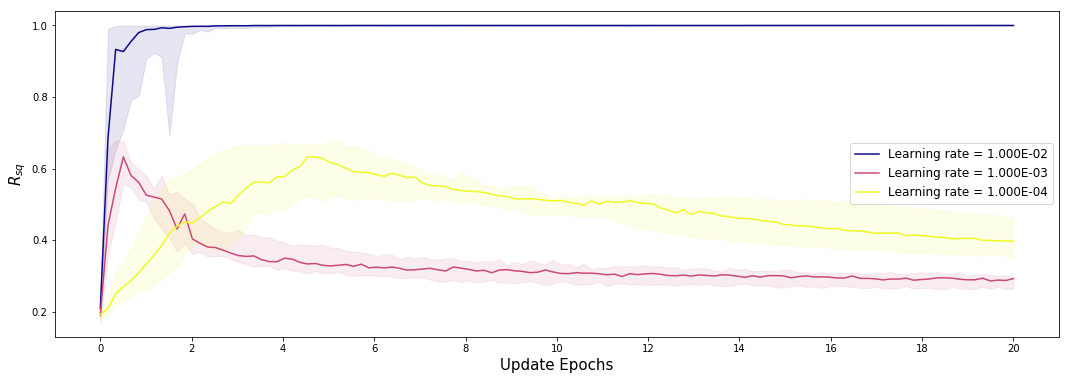
\includegraphics[width=\myWidth]{img/Sec5/sim1/dynamics_e20}
\caption[The dynamics of VNI $R_{sq}$ of the output layer.]
{
The dynamics of VNI $R_{sq}$ of the output layer.
The training is performed on the MNIST dataset 20 times, and then we evaluate the quartiles of the output VNI $R_{sq}$
for different learning rates.
Severe intensification of VNI (increases to 1 ) may occur as shown by the blue line which is trained with the learning rate of $10^{-2}$.
Otherwise VNI rises initially, and then decreases to a value which is larger than the initial VNI.
%It shows that overall, the correlation of each hidden layer is intensified during the back-propagation training. For large learning rate, the output VNI $R_{sq}$ severely increases to 1.
}
\label{fig:sec5_sim1}
\end{figure}
